\documentclass[11pt]{article}
\usepackage[top=1.00in, bottom=1.0in, left=1in, right=1in]{geometry}
\renewcommand{\baselinestretch}{1.1}
\usepackage{graphicx}
\usepackage{natbib}
\usepackage{amsmath}
\usepackage{parskip}
\usepackage{wrapfig}
\usepackage[font=small,labelfont=bf]{caption}
% counting words? https://app.uio.no/ifi/texcount/online.php

\def\labelitemi{--}
\parindent=0pt

\begin{document}
\bibliographystyle{/Users/Lizzie/Documents/EndnoteRelated/Bibtex/styles/ajhg}
\renewcommand{\refname}{\CHead{}}
% \setlength{\parindent}{0cm}
% \setlength{\parskip}{5pt}


{\bf Title:} Strengthening forest resilience through cross-disciplinary modeling of tree growth and decline across North America 

{\bf Funding for:} 24-week fellowship for E. M. Wolkovich of UBC  (Canada)  to visit Andrew Gelman at Columbia University (USA)

\begin{abstract}
Northern hemisphere forests are critical for healthy ecosystems, healthy people and drive the economies of many countries. They are also highly threatened by multiple risks, including climate change, pests and fire. While extensive research has worked to map and model these threats, the complexity of tree growth and the multi-scale and multi-threat nature of forest health has made understanding the major drivers of forest growth and decline difficult. Here, we propose a fellowship linking the University of British Columbia (Canada) with Columbia University (USA) to bridge across disciplines (ecology, statistics and climatology) for improved models of tree and forest health. Focusing on North American forests, we will model the complexity of tree growth at the individual level then use hierarchical modeling to integrate additional effects at the species, stand and regional levels to produce a continental understanding how, where and why forests are growing or declining. We expect this project will provide major new forecasts of tree growth and forest health, that can clearly separate out the effects of individual-level tree growth from stand level properties (e.g. species mixtures) and events (e.g., fire and pest outbreaks). Such forecasts can help improve large-scale modeling of the earth system and guide managers in how to manage forests for climate resiliency. 
\end{abstract}
% lu2015policy

\section*{Background}
\setlength{\intextsep}{6pt} 
\begin{wrapfigure}{r}{0.35\textwidth}
\centering
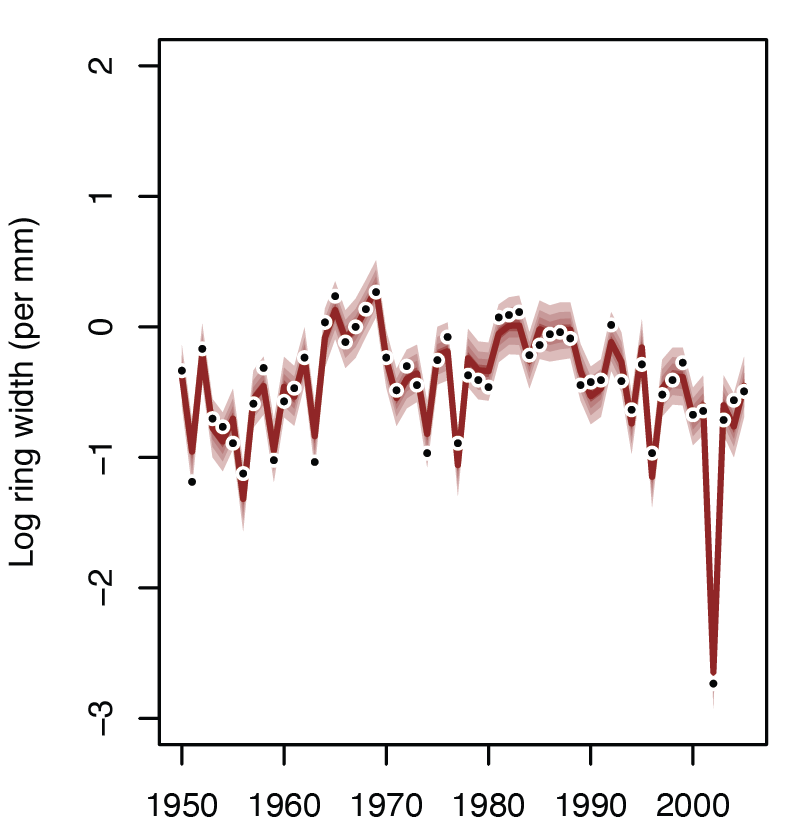
\includegraphics[width=0.33\textwidth]{figs/ut539_tree22_1panel.png}
\caption{An example of the complexity of tree growth from one \emph{Pinus ponderosa} tree sampled in Utah. Dots show the observed radial growth each year, while the coloring represents estimates from a hierarchical Gaussian process model.} 
\label{fig:onetree}
\end{wrapfigure}
Temperate forests across the globe provide critical resources for people \citep{oldekop2020forest,costanza2016sustainable}. Economically their timber underpins the economies of many states, provinces and countries, with their economic value increasing with climate change through their role as natural climate solutions increasing. Temperate forests currently sequester substantial fossil fuel emissions, offsetting planetary warming and acting as `natural climate solutions' \citep{pan2011large,griscom2017natural,friedlingstein2022global}.  The concept of natural climate solutions has increasingly recognized the role that forests play in carbon sequestration and other ecosystem services, including biodiversity maintenance and protection, water quality and stabilizing soils. 

Yet forests globally are threatened by multiple risks. In addition to forest loss and fragmentation, intact forests face potential declines due to climate change stress and the related threats of increasing wildfires and pest outbreaks \citep{trumbore2015forest}. Understanding, quantifying and forecasting these declines is clearly important to build resilience in forests and guide forest policy and management, but has been slow due to the inherent complexity of tree growth. 

Healthy resilient forests are an emergent property of individual-level tree growth, which is often highly variable and apparently difficult to predict (Fig. \ref{fig:onetree}). For these reasons, most work on radial tree growth to date has often worked from stand-level averages, after correcting for age-trends (tree-level allometry) \citep{cook1985time,Schofield2016}. This approach has been powerful for understanding the major role of climate in driving tree growth, and allowed global reconstructions of millennial-scale climate from tree growth patterns \citep{williams2020large}. Yet it has also made it difficult to identify the complex interactions that drive tree growth and thus forest health and decline. While recent work has begun to examine tree growth more in-depth, it has generally focused on only one species and region, limiting any relevance to larger scale forest management and policy.

Addressing these limitations requires a new approach to modeling forest health. It requires models that begin with modeling drivers of variability in the time-series of individual trees (Fig. \ref{fig:onetree}) and then build up to understand how different species and stands (sites) respond to climate and other factors. Such hierarchical (multi-level) models were previously difficult to fit across large, complex datasets, but advances in algorithms and methods \cite{hoffman2014no,Carpenter:2017stan}, alongside new data \citep{zhao2019international,pane2026spatial,williams2025western} have changed this reality. Here I (Wolkovich), working together with Gelman propose to apply these robust new approaches to data across North America to understand how tree growth and forests have shifted across North America in the last 130 years and project shifts in the future. 
% One of the leaders of these advances is Andrew Gelman
 \iffalse
* Why forests matter
* What's wrong with current forecasts?
	- Trees are complicated, to get around this, people lump them together... 
	- Signal-free issues
* What's needed
\fi 
\section*{Aims} 
Our objectives are threefold and build on one another: (1) Develop, test and refine hierarchical models of tree growth responses to climate, with approaches that can separate out species responses from stand and regional-level impacts; (2) estimate the impacts of pest outbreaks and fire relative to climate, by layering in newly available data at the stand-level on these events; (3) Forecast from these models with specific approaches to aid communication and dissemination of our results (described further under \emph{Expected outputs \& impact} below). 

 \iffalse
* Better models of growth responses to climate across species
	- separating out climate from species
* Dealing with tree and stand-level responses to elucidate pest and fire impacts
	- quantifying loss due to fire vs pest, versus climate change...
* New forecasts to guide forest management (planting after harvesting, regeneration after fire/pests)
\fi 

\section*{Methods}
This project will draw on data from the International Tree Ring Data Bank \citep{zhao2019international}, climate data from PRISM and NASA and new mapping efforts of fire and pest outbreaks to model tree growth across North America since 1896. We will add in additional tree ring data from the US Forest Inventory Analysis, CFS-TRenD repository and the BC Ministry of Forests as available. Dr. Benjamin Cook (NASA-GISS/Monash University) will assist in advance with finalizing tree ring and climate data. 

Working together with Gelman and colleagues, I will build from individual-level tree models of growth with age (allometry) to add in responses to annual climate with additional effects at the stand (or site) and regional levels. This multi-level approach will allow us to estimate the effect of different species, different climate, and events that occur at the stand-level, including fire and pest outbreaks. Following statistical workflow techniques pioneered by Gelman \citep{gelman2026bayesian}, we plan to fit an initial hierarchical model first, including climate responses (considering both linear and non-linear models) then test for whether stand-level differences are predictable based on pest and insect outbreaks. From there, we will integrate this information more fully into the models. % will develop the exact approach during the fellowship but we expect it

For climate, we plan to begin by focusing on summer warmth through growing degree days (GDD), moisture estimated through precipitation sums and stress effects possible through high vapor pressure deficit (VPD). Given the different climate drivers in western versus eastern North America, we plan a multi-step approach: we will fit western North America first where winter precipitation and VPD often dominate as drivers, then eastern North America where GDD is likely more important. 

Our focus on climate will be critical for forecasting from our model to predict how forests will respond to continuing anthropogenic climate change. These forecasts will be especially unique in providing guidance on how they may shift depending on future forest species and age composition and the management of fire and pest outbreaks. Our approach will yield a multi-level and multi-risk view, highlighting areas where management and policy could affect outcomes for more resilient forests.

\section*{Expected outputs \& impact}

Taken together we will deliver a cutting-edge new understanding of tree growth and forest change. Our resulting forecasts will be designed to help managers, policy-makers and other stakeholders understand the impacts of multiple risks in the future. These will include examining the impacts different future climate change scenarios (based on different fossil fuel emission levels), species planting regimes, and the scale of future wildfires and pest outbreaks. These forecasts and related visualizations can thus help guide different forest management decisions such as which species to plant after harvesting, and how to help regeneration after pests and fires depending on stand age and species composition (see also \emph{Contributions to CRP and action area}). 

We expect at least one major publication in a scientific journal from the work (e.g., \emph{Science, Nature Climate Change}) but possibly more depending on results and our interest in promoting our approach to other regions and multi-risk challenges. Thus, we expect we may have an additional manuscript to communicate how hierarchical models combined with forecasts and visualizations can aid managers and policymakers for agriculture, fisheries, and forestry. Finally, we expect the resulting collaboration (Wolkovich and Gelman) could have lasting impacts, with new projects on forest change resulting from this visit. We have long shared overlapping interests and perspectives, but not had the opportunity to collaborate before (see also \emph{Mutual benefits \& Hosting institutions}). 

\section*{Timeframe} % schedule/timeline
The fellowship is proposed for 15 September 2027 to 29 February 2028 (24 weeks) to bring Professor Elizabeth Wolkovich to Columbia University to work with Andrew Gelman and collaborators. If funded, we plan several videoconference meetings to discuss the aims, data and some modeling decisions in advance. Data collection and cleaning will then start before the fellowship to maximize the in-person time. While the project is ambitious, we (Wolkovich and Gelman) have worked together on the data and aims to make sure it is achievable within the 6-month time-frame and expect to have a report and at least one draft publication ready by the end of the CRP Fellowship. 

{\bf September 2027:} Finalize merging and cleaning tree ring and climate data. Gather mapping layers for forest pest and fire \citep{pane2026spatial,williams2025western}. Meetings to outline model approach.\\
{\bf October-November 2027:} Develop models, including code and checking, fit empirical data for North America (likely first to western areas, then extend to east).\\
{\bf December 2027:} Retrodictive checks for North America, and begin to work on visualizations for communication and dissemination.\\
{\bf January-February 2028:} Forecasting from model, including testing and finalizing visualizations for communication to stakeholders. Prepare publication and final report. 

\section*{Mutual benefits \& Hosting institutions}

We (Wolkovich and Gelman) have co-designed this project, drawing on our complementary skills sets and mutual interests, to maximize the benefits from it now and well into the future. Each will gain new knowledge and skills. I (Wolkovich) will learn advanced hierarchical modeling and forecast communication skills that I will bring back to UBC and the broader BC and Canadian communities. Gelman will gain an understanding of the forest health and carbon implications of tree growth from empirical data to forecasting that will help him work better with researchers across Columbia and beyond. Both Gelman and Wolkovich have extensive international collaborations where they can further share the knowledge and skills from this collaboration. I work extensively in France, Switzerland and the United Kingdom, while Gelman also works in France as well as Finland. 

Columbia's vibrant research community across the Departments of Statistics and Political Science---where Gelman is appointed---and the University's focus on cross-disciplinary earth system science through the Columbia Climate School and Lamont is uniquely positioned to support the proposed work and make sure it is well disseminated. Gelman himself is a rare researcher who fully combines scientific and statistical approaches to solve major challenges and then communicates them broadly. % While Gelman and Wolkovich have known each other through the statistical research community, they have only worked together briefly (and remotely) on a project on trophic synchrony. If funded, this fellowship would thus help launch their first major collaboration.   

\section*{Relevance to the selection criteria}

\subsection*{Contributions to CRP and action area}
The proposed work directly addresses the action area \emph{Addressing the action area of: strengthening resilience in the face of multiple risks in a connected world} with relevance also to \emph{innovating for sustainable production and productivity}. 
% Our focus on forests is a priority area for CRP with obvious extensions to other relevant topics, including soil, water, and biodiversity.  

Dealing with the uncertainty due to multiple risks of fires, pests and climate change in forests around the globe is critical, but limited by our understanding of what are the major drivers of forest growth versus decline. The proposed work will provide the best available information on the relative effect of different risk factors---climate change, pests, fire---at the same time it will estimate how intertwined they are. This information can in turn guide managers and other stakeholders in how to shape policy to prevent forest decline and thus increase carbon storage and mitigate climate change it self, given the global importance of North American forests to carbon storage. 

Our focus thus has global relevance for aiding forest and carbon policy on a global scale, but we will also leverage our focus on North American forests for impacts on state, provincial and national forests and forestry policies. We plan to focus on North American forests, many of which are highly managed for their timber and increasingly as natural climate solutions through their role in carbon sequestration. Given that forests cover much of the North American continent, they also broadly control biodiversity, water quality and soil stability and development. We discuss further the policy impacts of our proposed work below. 

\subsection*{Scientific excellence and innovation} 

This project is designed to reshape our understanding of tree growth and forest health, with lasting impacts on our scientific understanding and new approaches to understanding and communicating multiple risks for improved management and policy. Our work draws on extensive and vetted data on tree growth and climate, scaling from individual trees to continental scale analyses using cutting-edge methods. The proposer---Wolkovich---and host Gelman are both regarded as innovators in their field. Wolkovich has defined a new field of temporal ecology, with major implications from it for how we understand climate change and plant invasions, while Gelman has driven massive reform across different fields in developing better statistics, more reproducible approaches to science and understanding and exploiting the power or hierarchical models. He has a long track record of driving advances in different areas of science and will bring this focus to forest health. Wolkovich will bring cross-disciplinary expertise to Columbia, creating collaborations to develop better models of tree growth to strengthen and invigorate ties between the Columbia Climate School and Lamont Doherty Earth Observatory, while also building a lasting connection between UBC and Columbia. Beyond, this work could be innovative new approaches to multiple scales of communication and policy, as outlined below in \emph{Policy relevance}
% "This completion of these aims could be used as new supporting evidence and could be included in future OECD assessments" 

\section*{Feasibility}

Multiple aspects of our proposed work make it highly, including the scientific excellent and skills of Wolkovich and Gelman, as well as extensive work to compile data and design a plan that can be rapidly achieved. In addition to the excellence of Wolkovich and Gelman, additional collaborators have already pledge support the project with finalizing data (Dr. Cook, mentioned above) and helping with computational and modeling issues (Dr. Bob Carpenter). Columbia has agreed to provide all necessary support to make sure the project is a success, including office space, compute and additional resources as needed.%  extensions with Columbia Climate School etc. 

\subsection*{Scientific record and achievements of the proposer}

Wolkovich is a leading plant biology researcher who has defined and led the field of temporal ecology, focused on better understanding how biological time and climate shape plants, communities and ecosystem. Her work is highly cross-disciplinary, drawing on expertise from climatology and evolutionary biology, and very highly cited. She has over 80 peer-reviewed publications in high-impact journals (\emph{Nature, PNAS, Trends in Ecology \& Evolution, Ecology Letters}), with half of these cited 50 times or more (and several cited 500 or more times), of which she is first or senior author on over 70 of them. This ratio represents her focus on leading cutting-edge global research, which is highlighted by a recent collaborative lab meta-analysis that has resulted in publications in \emph{Nature Climate Change, New Phytologist, Global Change Biology}. Her research program routinely receives extensive media coverage, ranging from the \emph{Washington Post, Economist} and  \emph{USA Today} to interviews on BBC, NPR and CNN (see also \emph{Dissemination} below). 

\subsection*{Crossing disciplines}
This project is clearly cross-disciplinary, spanning biology, climatology and statistics. Wolkovich was trained in ecology, but draws on expertise from climatology and evolutionary biology. Gelman is a world-renowned expert in statistics and political science. Additional experts in climatology and computation methods (see also \emph{Feasibility}) have also pledged support. This cross-disciplinary approach is necessary to bring the level of scientific innovation and policy relevance for which the project is designed. 

\subsection*{Dissemination}
I (Wolkovich) and Gelman both have a history of being excellent communicators to diverse stakeholders. Gelman is extensively cited and interviewed in the mainstream media, and also maintains a widely read blog and Substack. Additionally, he is a widely appreciated expert on how to communicate and visualize statistics, including forecasts, contributing election forecasts---and how to communicate them---to \emph{The Economist} and other major outlets. Wolkovich's research in forestry and agriculture has to date has generated high interest, both in research and public spheres. For example, her lab's work on variety change with warming \cite{moralescastilla}, has been cited extensively and led to dozens of radio and print stories, including by the BBC, NPR, \emph{The Guardian, Washington Post, El Mundo} and France24 News. 

We will bring these skills to disseminating this work as well. We specifically plan to communicate results through publications, press releases and then at various conferences and and seminar series in which we are involved, including both in academic (e.g., universities), industry and non-profit (e.g., The Nature Conservancy and other organizations focused on Natural Climate Solutions) and government (e.g., BC Ministry of Forests) and through major international forums that cut across fields and domains (e.g., AGU). See also \emph{Expected outputs \& impact}.
% " country presentations to a series of end-users (from scientists, industry and policy makers)" 

\subsection*{Potential impact \& policy relevance}
% "This work will facilitate the exchange of science, knowledge "transfer and production of outreach activities to inform a wide range of end-users. 
This work is designed to reshape our understanding of forest growth and decline, with major impacts on how we manage forests and develop natural climate solutions. We expect this work will shift our fundamental understanding of how trees grow, yielding our best estimates of radial growth responses to temperature, VPD and precipitation---and how these climate impacts depend on and shift with pest outbreaks and fire. We expect this new outlook on tree growth will lead to new experiments, studies and drive new knowledge. Additionally, multiple aspects of our approach are designed to extend beyond. Our multi-scale approach can be extended both outward---to forests in other regions, countries and continents---and temporally downscaled, moving beyond annual resolution to potentially drawing on weekly or daily data (increasingly available through dendrometer networks). Our visualization and communication approach to forecasts from the model could be applied in other relevant OECD areas, especially agriculture. % See also \emph{Expected outputs \& impact}.

The same forest types and tree species occur across Canada and the United States, making connections in forest modeling and management between these countries important, especially with continuing climate change. This project will extend our understanding to improve forestry in both countries and natural climate solutions with global implications for climate and carbon modeling. Canada in particular has a series of programs for tree planting from the national level (through Natural Resources Canada) to the provincial level (especially BC Climate-Based Seed Transfer program), we which we expect this work will inform. Wolkovich has connections with these organizations and will make sure to work with them during and after the fellowship to share results for maximum impact. The US currently still has a Forest Service tree planting programs underway and the proposed work will be highly useful to New York state's 25 Million Trees by 2033. Our dissemination approach will work to inform and engage with  local stakeholders and managers to guide management in North American forests. Beyond North America, the carbon implications of our work have relevance to governance at the cross-country level of the OECD, the United Nations and similar organizations and we expect will shape knowledge documents and inform policy at this higher level. 

\section*{References}
\pagenumbering{gobble}
\def\section*#1{}
\bibliography{/Users/Lizzie/Documents/git/bibtex/LizzieMainMinimal}

\end{document}




\citep{ospreebbms}

\bibliographystyle{/Users/Lizzie/Documents/EndnoteRelated/Bibtex/styles/besjournals}
\bibliography{/Users/Lizzie/Documents/git/bibtex/LizzieMainMinimal}

\clearpage
\section{Figures}

\begin{figure}[h!]
\includegraphics[width=0.4\textwidth]{..//..//..//..//Professional/images/ColylusVineFruit2.png}
\caption{I am a caption.} 
\label{fig:figname}
\end{figure}'

% Find some relevant Canadian policies? Or just focus on BC? 
* -- Planting trees! % https://www.canada.ca/en/natural-resources-canada/news/2024/08/governments-of-canada-and-ontario-enhance-capacity-to-plant-trees-and-strengthen-ecosystems.html
* Natural Resources Canada -- How forests and forest products can help meet Canada’s climate goals % https://natural-resources.canada.ca/climate-change/climate-change-impacts-forests/forests-products-help-meet-canada-climate-goals
* (CBST) % https://www2.gov.bc.ca/gov/content/environment/natural-resource-stewardship/natural-resources-climate-change and genome BC https://www.genomebc.ca/blog/smart-reforestation-science-backed-policy-for-a-changing-climate/ ...
"This work directly informed the BC government’s Climate-Based Seed Transfer (CBST) policy, which became part of the Chief Forester’s Standards for Seed Use in 2018. " 
* US actually is still into this but that could change in a moment ... % https://www.fs.usda.gov/managing-land/sc/policy-initiatives
* New York is super into this ... 25 Million Trees by 2033 % https://dec.ny.gov/nature/forests-trees/climate-change/25-million-trees



